% Created by tikzDevice version 0.12.3.1 on 2021-02-23 15:47:20
% !TEX encoding = UTF-8 Unicode
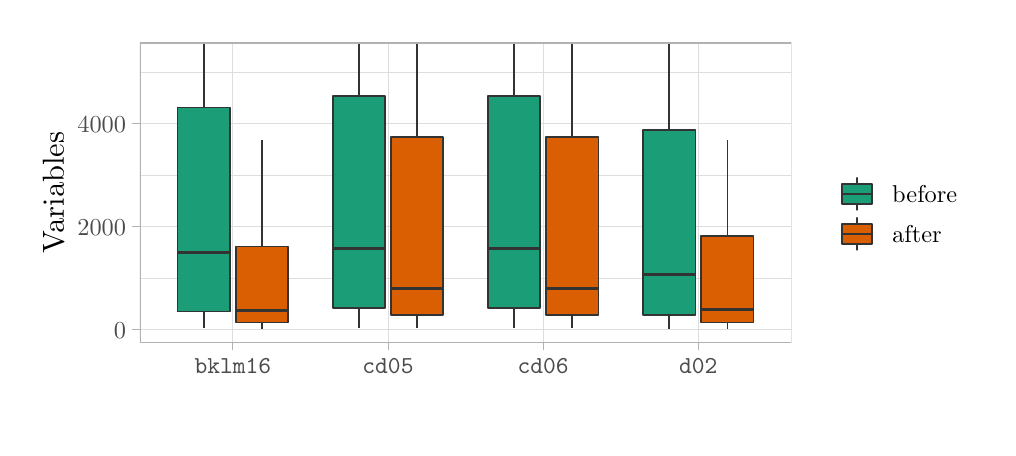
\begin{tikzpicture}[x=1pt,y=1pt]
\definecolor{fillColor}{RGB}{255,255,255}
\path[use as bounding box,fill=fillColor,fill opacity=0.00] (0,0) rectangle (346.90,144.54);
\begin{scope}
\path[clip] (  0.00,  0.00) rectangle (346.90,144.54);
\definecolor{drawColor}{RGB}{255,255,255}
\definecolor{fillColor}{RGB}{255,255,255}

\path[draw=drawColor,line width= 0.6pt,line join=round,line cap=round,fill=fillColor] (  0.00,  0.00) rectangle (346.90,144.54);
\end{scope}
\begin{scope}
\path[clip] ( 40.51, 30.69) rectangle (275.96,139.04);
\definecolor{fillColor}{RGB}{255,255,255}

\path[fill=fillColor] ( 40.51, 30.69) rectangle (275.96,139.04);
\definecolor{drawColor}{gray}{0.87}

\path[draw=drawColor,line width= 0.1pt,line join=round] ( 40.51, 54.03) --
	(275.96, 54.03);

\path[draw=drawColor,line width= 0.1pt,line join=round] ( 40.51, 91.24) --
	(275.96, 91.24);

\path[draw=drawColor,line width= 0.1pt,line join=round] ( 40.51,128.46) --
	(275.96,128.46);

\path[draw=drawColor,line width= 0.3pt,line join=round] ( 40.51, 35.42) --
	(275.96, 35.42);

\path[draw=drawColor,line width= 0.3pt,line join=round] ( 40.51, 72.64) --
	(275.96, 72.64);

\path[draw=drawColor,line width= 0.3pt,line join=round] ( 40.51,109.85) --
	(275.96,109.85);

\path[draw=drawColor,line width= 0.3pt,line join=round] ( 74.15, 30.69) --
	( 74.15,139.04);

\path[draw=drawColor,line width= 0.3pt,line join=round] (130.20, 30.69) --
	(130.20,139.04);

\path[draw=drawColor,line width= 0.3pt,line join=round] (186.26, 30.69) --
	(186.26,139.04);

\path[draw=drawColor,line width= 0.3pt,line join=round] (242.32, 30.69) --
	(242.32,139.04);
\definecolor{drawColor}{gray}{0.20}

\path[draw=drawColor,line width= 0.6pt,line join=round] ( 63.63,115.66) -- ( 63.63,144.54);

\path[draw=drawColor,line width= 0.6pt,line join=round] ( 63.63, 41.94) -- ( 63.63, 35.91);
\definecolor{fillColor}{RGB}{27,158,119}

\path[draw=drawColor,line width= 0.6pt,line join=round,line cap=round,fill=fillColor] ( 54.17,115.66) --
	( 54.17, 41.94) --
	( 73.09, 41.94) --
	( 73.09,115.66) --
	( 54.17,115.66) --
	cycle;

\path[draw=drawColor,line width= 1.1pt,line join=round] ( 54.17, 63.32) -- ( 73.09, 63.32);

\path[draw=drawColor,line width= 0.6pt,line join=round] ( 84.66, 65.49) -- ( 84.66,104.12);

\path[draw=drawColor,line width= 0.6pt,line join=round] ( 84.66, 38.03) -- ( 84.66, 35.61);
\definecolor{fillColor}{RGB}{217,95,2}

\path[draw=drawColor,line width= 0.6pt,line join=round,line cap=round,fill=fillColor] ( 75.20, 65.49) --
	( 75.20, 38.03) --
	( 94.12, 38.03) --
	( 94.12, 65.49) --
	( 75.20, 65.49) --
	cycle;

\path[draw=drawColor,line width= 1.1pt,line join=round] ( 75.20, 42.42) -- ( 94.12, 42.42);

\path[draw=drawColor,line width= 0.6pt,line join=round] (119.69,119.81) -- (119.69,144.54);

\path[draw=drawColor,line width= 0.6pt,line join=round] (119.69, 43.24) -- (119.69, 36.02);
\definecolor{fillColor}{RGB}{27,158,119}

\path[draw=drawColor,line width= 0.6pt,line join=round,line cap=round,fill=fillColor] (110.23,119.81) --
	(110.23, 43.24) --
	(129.15, 43.24) --
	(129.15,119.81) --
	(110.23,119.81) --
	cycle;

\path[draw=drawColor,line width= 1.1pt,line join=round] (110.23, 64.90) -- (129.15, 64.90);

\path[draw=drawColor,line width= 0.6pt,line join=round] (140.71,104.94) -- (140.71,144.54);

\path[draw=drawColor,line width= 0.6pt,line join=round] (140.71, 40.63) -- (140.71, 35.85);
\definecolor{fillColor}{RGB}{217,95,2}

\path[draw=drawColor,line width= 0.6pt,line join=round,line cap=round,fill=fillColor] (131.26,104.94) --
	(131.26, 40.63) --
	(150.17, 40.63) --
	(150.17,104.94) --
	(131.26,104.94) --
	cycle;

\path[draw=drawColor,line width= 1.1pt,line join=round] (131.26, 50.31) -- (150.17, 50.31);

\path[draw=drawColor,line width= 0.6pt,line join=round] (175.75,119.86) -- (175.75,144.54);

\path[draw=drawColor,line width= 0.6pt,line join=round] (175.75, 43.24) -- (175.75, 36.02);
\definecolor{fillColor}{RGB}{27,158,119}

\path[draw=drawColor,line width= 0.6pt,line join=round,line cap=round,fill=fillColor] (166.29,119.86) --
	(166.29, 43.24) --
	(185.21, 43.24) --
	(185.21,119.86) --
	(166.29,119.86) --
	cycle;

\path[draw=drawColor,line width= 1.1pt,line join=round] (166.29, 64.90) -- (185.21, 64.90);

\path[draw=drawColor,line width= 0.6pt,line join=round] (196.77,104.94) -- (196.77,144.54);

\path[draw=drawColor,line width= 0.6pt,line join=round] (196.77, 40.63) -- (196.77, 35.85);
\definecolor{fillColor}{RGB}{217,95,2}

\path[draw=drawColor,line width= 0.6pt,line join=round,line cap=round,fill=fillColor] (187.31,104.94) --
	(187.31, 40.63) --
	(206.23, 40.63) --
	(206.23,104.94) --
	(187.31,104.94) --
	cycle;

\path[draw=drawColor,line width= 1.1pt,line join=round] (187.31, 50.31) -- (206.23, 50.31);

\path[draw=drawColor,line width= 0.6pt,line join=round] (231.81,107.47) -- (231.81,144.54);

\path[draw=drawColor,line width= 0.6pt,line join=round] (231.81, 40.63) -- (231.81, 35.83);
\definecolor{fillColor}{RGB}{27,158,119}

\path[draw=drawColor,line width= 0.6pt,line join=round,line cap=round,fill=fillColor] (222.35,107.47) --
	(222.35, 40.63) --
	(241.27, 40.63) --
	(241.27,107.47) --
	(222.35,107.47) --
	cycle;

\path[draw=drawColor,line width= 1.1pt,line join=round] (222.35, 55.32) -- (241.27, 55.32);

\path[draw=drawColor,line width= 0.6pt,line join=round] (252.83, 69.18) -- (252.83,104.12);

\path[draw=drawColor,line width= 0.6pt,line join=round] (252.83, 38.03) -- (252.83, 35.61);
\definecolor{fillColor}{RGB}{217,95,2}

\path[draw=drawColor,line width= 0.6pt,line join=round,line cap=round,fill=fillColor] (243.37, 69.18) --
	(243.37, 38.03) --
	(262.29, 38.03) --
	(262.29, 69.18) --
	(243.37, 69.18) --
	cycle;

\path[draw=drawColor,line width= 1.1pt,line join=round] (243.37, 42.87) -- (262.29, 42.87);
\definecolor{drawColor}{gray}{0.70}

\path[draw=drawColor,line width= 0.6pt,line join=round,line cap=round] ( 40.51, 30.69) rectangle (275.96,139.04);
\end{scope}
\begin{scope}
\path[clip] (  0.00,  0.00) rectangle (346.90,144.54);
\definecolor{drawColor}{gray}{0.30}

\node[text=drawColor,anchor=base east,inner sep=0pt, outer sep=0pt, scale=  0.88] at ( 35.56, 32.39) {0};

\node[text=drawColor,anchor=base east,inner sep=0pt, outer sep=0pt, scale=  0.88] at ( 35.56, 69.61) {2000};

\node[text=drawColor,anchor=base east,inner sep=0pt, outer sep=0pt, scale=  0.88] at ( 35.56,106.82) {4000};
\end{scope}
\begin{scope}
\path[clip] (  0.00,  0.00) rectangle (346.90,144.54);
\definecolor{drawColor}{gray}{0.70}

\path[draw=drawColor,line width= 0.3pt,line join=round] ( 37.76, 35.42) --
	( 40.51, 35.42);

\path[draw=drawColor,line width= 0.3pt,line join=round] ( 37.76, 72.64) --
	( 40.51, 72.64);

\path[draw=drawColor,line width= 0.3pt,line join=round] ( 37.76,109.85) --
	( 40.51,109.85);
\end{scope}
\begin{scope}
\path[clip] (  0.00,  0.00) rectangle (346.90,144.54);
\definecolor{drawColor}{gray}{0.70}

\path[draw=drawColor,line width= 0.3pt,line join=round] ( 74.15, 27.94) --
	( 74.15, 30.69);

\path[draw=drawColor,line width= 0.3pt,line join=round] (130.20, 27.94) --
	(130.20, 30.69);

\path[draw=drawColor,line width= 0.3pt,line join=round] (186.26, 27.94) --
	(186.26, 30.69);

\path[draw=drawColor,line width= 0.3pt,line join=round] (242.32, 27.94) --
	(242.32, 30.69);
\end{scope}
\begin{scope}
\path[clip] (  0.00,  0.00) rectangle (346.90,144.54);
\definecolor{drawColor}{gray}{0.30}

\node[text=drawColor,anchor=base,inner sep=0pt, outer sep=0pt, scale=  0.88] at ( 74.15, 19.68) {\texttt{bklm16}};

\node[text=drawColor,anchor=base,inner sep=0pt, outer sep=0pt, scale=  0.88] at (130.20, 19.68) {\texttt{cd05}};

\node[text=drawColor,anchor=base,inner sep=0pt, outer sep=0pt, scale=  0.88] at (186.26, 19.68) {\texttt{cd06}};

\node[text=drawColor,anchor=base,inner sep=0pt, outer sep=0pt, scale=  0.88] at (242.32, 19.68) {\texttt{d02}};
\end{scope}
\begin{scope}
\path[clip] (  0.00,  0.00) rectangle (346.90,144.54);
\definecolor{drawColor}{RGB}{0,0,0}

\node[text=drawColor,rotate= 90.00,anchor=base,inner sep=0pt, outer sep=0pt, scale=  1.10] at ( 13.08, 84.86) {Variables};
\end{scope}
\begin{scope}
\path[clip] (  0.00,  0.00) rectangle (346.90,144.54);
\definecolor{fillColor}{RGB}{255,255,255}

\path[fill=fillColor] (286.96, 57.30) rectangle (341.40,112.42);
\end{scope}
\begin{scope}
\path[clip] (  0.00,  0.00) rectangle (346.90,144.54);
\definecolor{fillColor}{RGB}{255,255,255}

\path[fill=fillColor] (292.46, 77.26) rectangle (306.91, 91.71);
\end{scope}
\begin{scope}
\path[clip] (  0.00,  0.00) rectangle (346.90,144.54);
\definecolor{drawColor}{gray}{0.20}

\path[draw=drawColor,line width= 0.6pt,line join=round,line cap=round] (299.68, 78.70) --
	(299.68, 80.87);

\path[draw=drawColor,line width= 0.6pt,line join=round,line cap=round] (299.68, 88.10) --
	(299.68, 90.26);
\definecolor{fillColor}{RGB}{27,158,119}

\path[draw=drawColor,line width= 0.6pt,line join=round,line cap=round,fill=fillColor] (294.26, 80.87) rectangle (305.10, 88.10);

\path[draw=drawColor,line width= 0.6pt,line join=round,line cap=round] (294.26, 84.48) --
	(305.10, 84.48);
\end{scope}
\begin{scope}
\path[clip] (  0.00,  0.00) rectangle (346.90,144.54);
\definecolor{fillColor}{RGB}{255,255,255}

\path[fill=fillColor] (292.46, 62.80) rectangle (306.91, 77.26);
\end{scope}
\begin{scope}
\path[clip] (  0.00,  0.00) rectangle (346.90,144.54);
\definecolor{drawColor}{gray}{0.20}

\path[draw=drawColor,line width= 0.6pt,line join=round,line cap=round] (299.68, 64.25) --
	(299.68, 66.42);

\path[draw=drawColor,line width= 0.6pt,line join=round,line cap=round] (299.68, 73.64) --
	(299.68, 75.81);
\definecolor{fillColor}{RGB}{217,95,2}

\path[draw=drawColor,line width= 0.6pt,line join=round,line cap=round,fill=fillColor] (294.26, 66.42) rectangle (305.10, 73.64);

\path[draw=drawColor,line width= 0.6pt,line join=round,line cap=round] (294.26, 70.03) --
	(305.10, 70.03);
\end{scope}
\begin{scope}
\path[clip] (  0.00,  0.00) rectangle (346.90,144.54);
\definecolor{drawColor}{RGB}{0,0,0}

\node[text=drawColor,anchor=base west,inner sep=0pt, outer sep=0pt, scale=  0.88] at (312.41, 81.45) {before};
\end{scope}
\begin{scope}
\path[clip] (  0.00,  0.00) rectangle (346.90,144.54);
\definecolor{drawColor}{RGB}{0,0,0}

\node[text=drawColor,anchor=base west,inner sep=0pt, outer sep=0pt, scale=  0.88] at (312.41, 67.00) {after};
\end{scope}
\end{tikzpicture}
